\section{Monetary Policy: Rules vs Discretion (Barro-Gordon)}

\subsection{Rules vs discretion and the inflation bias \pg{88}}

\paragraph{Two ways to conduct policy.}
\begin{itemize}
  \item \textbf{Discretion:} policy is chosen \emph{period by period}. Each period the central bank (CB) picks the best action given the current situation, with no necessary connection between the choices made in different periods. In particular, it cannot bind its future self.
  \item \textbf{Rule:} the CB follows a \emph{formula} describing policy over a large number of periods, and commits to it in advance (before the public forms its expectations).
\end{itemize}

\begin{keybox}[title=Kydland--Prescott result]
Discretionary policymaking produces an \textbf{inflation bias}: the equilibrium inflation rate exceeds the socially desired inflation rate, without any gain in output.
\end{keybox}

\paragraph{Where does the bias come from?} Two ingredients are needed together.
\begin{enumerate}
  \item \textbf{The CB wants output above potential} (equivalently, unemployment below the natural rate).
  \begin{itemize}
    \item \emph{Potential output} is the highest output the economy can produce with resources fully used and without creating inflationary pressure.
    \item The \emph{natural rate of unemployment} is the unemployment rate in the market's long-run equilibrium.
    \item The CB is tempted to push output above potential by stimulating demand, e.g.\ by raising money growth.
  \end{itemize}
  \item \textbf{The CB cannot credibly commit to low inflation.} If firms and workers do not believe the CB will keep inflation low, they expect higher inflation and set wages and prices accordingly. Higher expected inflation then shows up as higher actual inflation.
\end{enumerate}
Interpretation: the public knows the CB is tempted to inflate, so it builds that inflation into its expectations in advance. The CB ends up delivering the expected (high) inflation simply to avoid an output loss, and output is no higher than it would have been with low inflation.

\subsection{AD--AS view of a monetary expansion \pg{88--89}}

\paragraph{Setup.}
\begin{itemize}
  \item $P$: price level; $y$: aggregate output; $y^*$: potential (natural) output.
  \item AD: aggregate demand curve, downward sloping in $(y,P)$. A monetary expansion shifts it to the right.
  \item SRAS: short-run aggregate supply, upward sloping because \emph{nominal} wages $w$ are fixed in the short run: a higher $P$ lowers the real wage $w/P$, so firms hire more labour $L$ and produce more.
  \item LRAS: long-run aggregate supply, vertical at $y^*$, since in the long run nominal wages fully adjust and the real wage returns to its market-clearing level.
\end{itemize}

\begin{center}
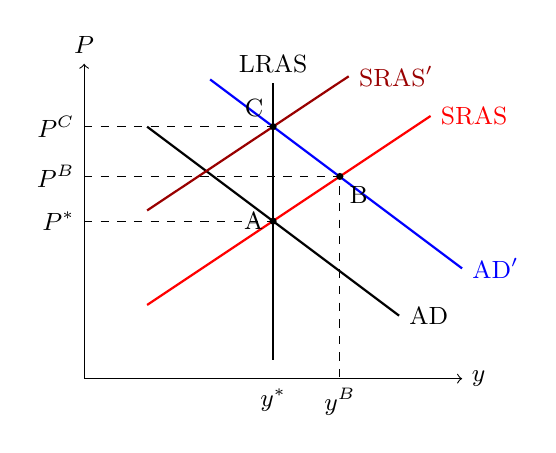
\begin{tikzpicture}[scale=0.8,font=\small]
  \draw[->] (0,0)--(6,0) node[right]{$y$};
  \draw[->] (0,0)--(0,5) node[above]{$P$};
  \draw[thick] (3,0.3)--(3,4.7) node[above]{LRAS};
  \draw[thick] (1,4)--(5,1) node[right]{AD};
  \draw[thick,blue] (2,4.75)--(6,1.75) node[right]{AD$'$};
  \draw[thick,red] (1,1.17)--(5.5,4.17) node[right]{SRAS};
  \draw[thick,red!60!black] (1,2.67)--(4.2,4.8) node[right]{SRAS$'$};
  \fill (3,2.5) circle (1.6pt) node[left]{A};
  \fill (4.06,3.21) circle (1.6pt) node[below right]{B};
  \fill (3,4) circle (1.6pt) node[above left]{C};
  \draw[dashed] (0,2.5) node[left]{$P^*$}--(3,2.5);
  \draw[dashed] (0,3.21) node[left]{$P^B$}--(4.06,3.21)--(4.06,0) node[below]{$y^B$};
  \draw[dashed] (0,4) node[left]{$P^C$}--(3,4);
  \node[below] at (3,0) {$y^*$};
\end{tikzpicture}
\end{center}
\emph{How to read the figure.} Output is on the horizontal axis and the price level on the vertical axis. The economy starts at A, where AD, SRAS and LRAS all cross. The expansion moves AD to the right (blue line), so the short-run equilibrium is B, on the old SRAS. Once nominal wages adjust, SRAS shifts up and to the left (dark red line), and the economy ends at C: back on LRAS, with a higher price level.

\paragraph{Step by step.}
\begin{itemize}
  \item \textbf{Initial equilibrium (A):} AD crosses SRAS on the LRAS line, at $(y^*,P^*)$. The economy is stable and no policy is changing.
  \item \textbf{Short run (A$\to$B):} the monetary expansion shifts AD to AD$'$, raising demand for goods and services. Along the old SRAS, with nominal wages fixed:
  \[
  P\uparrow\ \Rightarrow\ \frac{w}{P}\downarrow\ \Rightarrow\ \text{hiring is cheaper, } L\uparrow\ \Rightarrow\ y\uparrow .
  \]
  Price rises from $P^*$ to $P^B$ and output from $y^*$ to $y^B>y^*$.
  \item \textbf{Long run (B$\to$C):} over time workers see that the price level has risen and ask for higher nominal wages $w$ to protect their purchasing power. As $w$ rises, the real wage $w/P$ goes back to its original level. Labour costs rise, so SRAS shifts left to SRAS$'$:
  \[
  w\uparrow\ \Rightarrow\ \frac{w}{P}\uparrow \text{ (back to original)}\ \Rightarrow\ L\downarrow\ \Rightarrow\ y\downarrow \text{ back to } y^*,\qquad P\uparrow \text{ further to } P^C .
  \]
  \item \textbf{Outcome:} the price level is permanently higher ($P^C>P^B>P^*$), but output is back at potential $y^*$.
\end{itemize}
\begin{tipbox}
A demand shock (such as a monetary expansion) has real effects only when there is a market imperfection, here sticky nominal wages. Without such an imperfection, a demand shock only moves prices. In the long run: higher $P$, same $y^*$. This short-run real effect is exactly what tempts the CB in the Barro--Gordon model below.
\end{tipbox}

\subsection{Barro--Gordon model: setup \pg{89--91}}

\paragraph{Overview.} A static (one-period) model with a central bank and a private sector (workers and firms) that has rational expectations. The CB chooses money growth; the public chooses its inflation expectation (through nominal wage contracts) \emph{before} the CB acts.

\paragraph{Variables and parameters.}
\begin{itemize}
  \item $y$: actual output; $y_n$: natural (market-clearing) level of output.
  \item $\pi$: actual inflation rate; $\pi^e$: inflation rate expected by the public; $\bar\pi$: socially optimal inflation rate, assumed $\bar\pi=0$.
  \item $k>0$: political-pressure parameter. The CB's output target is $y_n+k$, i.e.\ \emph{above} the natural level.
  \item $\lambda>0$: weight the CB puts on output stabilization relative to price stabilization.
  \item $a>0$: sensitivity of output to inflation surprises $\pi-\pi^e$.
  \item $\Delta M$: growth rate of the money supply (the CB's instrument).
  \item $e$: supply shock; $v$: price (inflation) shock. Both have mean zero, are uncorrelated, and have variances $\sigma_e^2,\sigma_v^2$:
  \[
  E[e]=E[v]=0,\qquad E[ev]=E[e]E[v]=0,\qquad E[e^2]=\sigma_e^2,\qquad E[v^2]=\sigma_v^2 .
  \]
\end{itemize}

\paragraph{CB loss function.} The CB minimizes the expected value of
\begin{equation}
V=\tfrac12\lambda\,(y-y_n-k)^2+\tfrac12(\pi-\bar\pi)^2,\qquad \bar\pi=0 .\label{eq:bg-loss}
\end{equation}
The first term penalizes deviations of output from the target $y_n+k$; the second penalizes deviations of inflation from $0$. So the CB's problem is to stabilize $y$ around $y_n+k$ and $\pi$ around $0$.

\paragraph{Aggregate supply (expectations-augmented / Lucas supply).}
\begin{equation}
y=y_n+a(\pi-\pi^e)+e .\label{eq:bg-as}
\end{equation}
\begin{itemize}
  \item \textbf{Motivation:} wages are set in \emph{nominal} terms in one-period contracts, based on $\pi^e$. If actual inflation is higher than expected ($\pi>\pi^e$), prices rise faster than workers anticipated, the real wage is eroded, firms hire more workers and output rises above $y_n$. Only \emph{surprise} inflation raises output.
  \item $e$ is a supply shock that shifts aggregate supply left or right, e.g.\ a sharp rise in the price of a key input such as oil (a negative $e$).
\end{itemize}

\paragraph{Inflation.} The CB controls money growth but not inflation exactly:
\begin{equation}
\pi=\Delta M+v .\label{eq:bg-pi}
\end{equation}
The price shock $v$ means the CB cannot fully control $\pi$.

\paragraph{Timing of events.}
\begin{center}
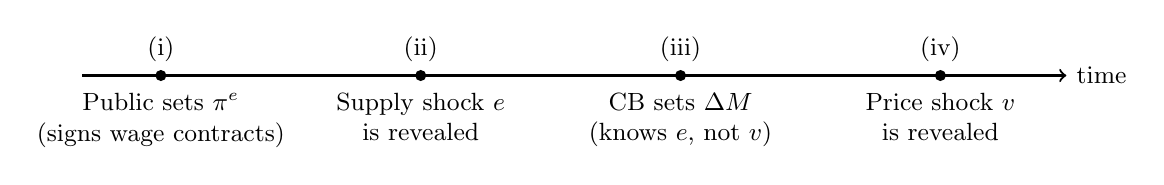
\begin{tikzpicture}[font=\small,x=1cm]
  \draw[->,thick] (0,0)--(12.5,0) node[right]{time};
  \foreach \x/\lab/\txt in {1/(i)/{Public sets $\pi^e$\\(signs wage contracts)},4.3/(ii)/{Supply shock $e$\\is revealed},7.6/(iii)/{CB sets $\Delta M$\\(knows $e$, not $v$)},10.9/(iv)/{Price shock $v$\\is revealed}}{
    \fill (\x,0) circle (2pt);
    \node[above] at (\x,0.05) {\lab};
    \node[below,align=center] at (\x,-0.1) {\txt};
  }
\end{tikzpicture}
\end{center}
Read the timeline left to right. Expectations are locked in first, so when the CB moves at stage (iii), $\pi^e$ is already fixed and the CB takes it as given. The CB can respond to $e$, which it has seen, but not to $v$, which is revealed only after it acts. So the public faces shocks and rigid wage contracts, and the CB uses monetary policy to stabilize output and inflation.

\paragraph{The loss in terms of the CB's instrument.} Substitute \eqref{eq:bg-as} into \eqref{eq:bg-loss}, using $\bar\pi=0$. Since $y-y_n=a(\pi-\pi^e)+e$,
\begin{equation}
V=\tfrac12\lambda\big[a(\pi-\pi^e)+e-k\big]^2+\tfrac12\pi^2 .\label{eq:bg-loss-pi}
\end{equation}
Now substitute $\pi=\Delta M+v$ from \eqref{eq:bg-pi} and expand $a(\pi-\pi^e)=a\Delta M+av-a\pi^e$:
\begin{equation}
V=\tfrac12\lambda\big[a\Delta M+av-a\pi^e+e-k\big]^2+\tfrac12(\Delta M+v)^2 .\label{eq:bg-loss-dm}
\end{equation}
How $\Delta M$ is chosen differs between discretion and a rule; that is the whole point of the comparison below.

\subsection{Equilibrium under discretion \pg{91--93}}

\paragraph{Solution strategy (backward induction).}
\begin{enumerate}
  \item Solve the CB's problem at stage (iii), taking $\pi^e$ and $e$ as given: this gives $\Delta M$ as a function of $(\pi^e,e)$.
  \item Go back to stage (i): the public, knowing this reaction function, forms rational expectations $\pi^e=E[\pi]$.
  \item Substitute $\pi^e$ back to get equilibrium $\Delta M$, $\pi$, output, and the expected loss.
\end{enumerate}

\paragraph{Step 1: the CB's problem.} Having observed $e$, and with $\pi^e$ already fixed, the CB solves
\[
\min_{\Delta M}\ E\{V\mid e\},
\]
where $V$ is \eqref{eq:bg-loss-dm} and the expectation is over the unknown $v$ only.

We use the chain rule, $\frac{d}{dx}\tfrac12 f(x)^2=f(x)f'(x)$, and the fact that we may differentiate inside the expectation. The derivative of the first term of \eqref{eq:bg-loss-dm} with respect to $\Delta M$ is $\lambda[\cdot]\cdot a$; the derivative of the second is $(\Delta M+v)$. The first-order condition (FOC) is
\begin{align*}
&E\big\{\lambda\big(a\Delta M+av-a\pi^e+e-k\big)a+\Delta M+v\ \big|\ e\big\}=0\\
\intertext{Multiply out the first term ($e$, $\pi^e$, $\Delta M$ are known, so only $v$ is random):}
&\lambda a^2\Delta M+\lambda a^2E[v]-\lambda a^2\pi^e+\lambda a e-\lambda a k+\Delta M+E[v]=0\\
\intertext{Use $E[v]=0$ and group the terms:}
&\lambda a^2\Delta M+\Delta M=\lambda a^2\pi^e+\lambda a(k-e)\\
\intertext{Factor out $\Delta M$:}
&(1+\lambda a^2)\,\Delta M=\lambda a^2\pi^e+\lambda a(k-e).
\end{align*}
The second-order condition holds since $\partial^2 V/\partial(\Delta M)^2=\lambda a^2+1>0$. Divide by $1+\lambda a^2$:
\begin{equation}
\Delta M=\frac{\lambda a^2\pi^e+\lambda a(k-e)}{1+\lambda a^2}.\label{eq:bg-dm}
\end{equation}
Interpretation of \eqref{eq:bg-dm}:
\begin{itemize}
  \item \textbf{Policy depends on the realized supply shock $e$.} A bad supply shock ($e<0$) lowers output and raises $\Delta M$ to offset it. Offsetting it fully would cost inflation, so the CB faces a \emph{trade-off} between stabilizing output and stabilizing inflation.
  \item \textbf{Optimal policy depends on $\pi^e$.} Higher expected inflation lowers output for a given $\pi$, so the CB partly accommodates it with more money growth.
\end{itemize}

\paragraph{The reaction function (special case $e=v=0$).} With no shocks, $\pi=\Delta M$ and \eqref{eq:bg-dm} becomes
\begin{equation}
\pi=\Delta M=\frac{\lambda a^2}{1+\lambda a^2}\,\pi^e+\frac{\lambda a}{1+\lambda a^2}\,k .\label{eq:bg-react}
\end{equation}
\begin{center}
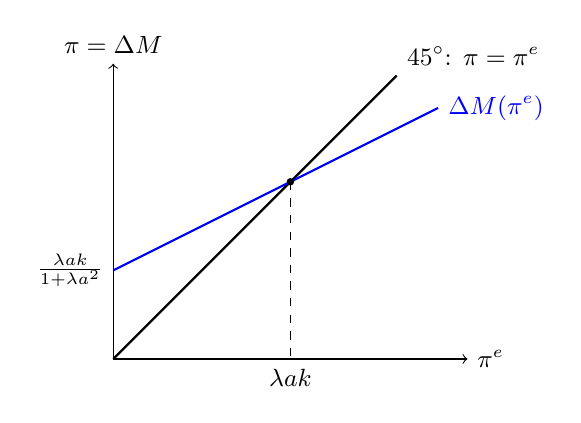
\begin{tikzpicture}[scale=0.75,font=\small]
  \draw[->] (0,0)--(6,0) node[right]{$\pi^e$};
  \draw[->] (0,0)--(0,5) node[above]{$\pi=\Delta M$};
  \draw[thick] (0,0)--(4.8,4.8) node[above right]{$45^\circ$: $\pi=\pi^e$};
  \draw[thick,blue] (0,1.5)--(5.5,4.25) node[right]{$\Delta M(\pi^e)$};
  \node[left] at (0,1.5) {$\frac{\lambda a k}{1+\lambda a^2}$};
  \fill (3,3) circle (1.8pt);
  \draw[dashed] (3,3)--(3,0) node[below]{$\lambda a k$};
\end{tikzpicture}
\end{center}
\emph{How to read the figure.} The horizontal axis is expected inflation and the vertical axis is the inflation the CB chooses. The blue line is the CB's best response \eqref{eq:bg-react}. Along the $45^\circ$ line, actual inflation equals expected inflation, which must hold in an equilibrium without shocks. The equilibrium is where the two lines cross.
\begin{itemize}
  \item \textbf{Intercept} $\frac{\lambda ak}{1+\lambda a^2}>0$ when $k>0$: even if the public expects zero inflation, the CB inflates.
  \item \textbf{Slope} $\frac{\lambda a^2}{1+\lambda a^2}<1$: the line is flatter than the $45^\circ$ line. The CB does not fully match an increase in expectations with money growth, because it also cares about inflation itself. The flatter the slope, the more weight it puts on inflation relative to output.
  \item \textbf{If $\pi^e=0$:} $\Delta M=\frac{\lambda a}{1+\lambda a^2}k$, which depends only on the political pressure $k$. If $k=0$, then $\Delta M=0$; if $k>0$, the CB raises $\Delta M$. So with $k>0$, $\pi^e=0$ \emph{cannot} be an equilibrium: the public would be surprised every time.
\end{itemize}

\paragraph{Step 2: rational expectations.} The public moves first and understands the CB's incentives, so it uses \eqref{eq:bg-dm} to form its expectation. It cannot predict $e$ or $v$, and both have mean zero. Rational expectations means $\pi^e=E[\pi]$:
\begin{align*}
\pi^e&=E[\pi]=E[\Delta M+v]=E[\Delta M] &&\text{(by \eqref{eq:bg-pi} and $E[v]=0$)}\\
&=\frac{\lambda a^2\pi^e+\lambda a(k-E[e])}{1+\lambda a^2} &&\text{(take expectations of \eqref{eq:bg-dm})}\\
&=\frac{\lambda a^2\pi^e+\lambda ak}{1+\lambda a^2} &&\text{(use $E[e]=0$).}
\end{align*}
Solve this for $\pi^e$. Multiply both sides by $1+\lambda a^2$:
\begin{align*}
(1+\lambda a^2)\pi^e&=\lambda a^2\pi^e+\lambda ak\\
\intertext{Subtract $\lambda a^2\pi^e$ from both sides:}
\pi^e&=\lambda ak .
\end{align*}
\begin{equation}
\boxed{\pi^e=\lambda ak>0}\label{eq:bg-pie}
\end{equation}
Expected inflation increases with $\lambda$ (more weight on output), with $a$ (surprises are more effective) and with $k$ (more ambitious output target). This is the crossing point in the figure: plugging $\pi^e=\lambda ak$ into \eqref{eq:bg-react} gives back $\pi=\lambda ak$.

\paragraph{Step 3: equilibrium money growth and inflation.} Substitute \eqref{eq:bg-pie} into \eqref{eq:bg-dm}:
\begin{align*}
\Delta M^D&=\frac{\lambda a^2(\lambda ak)+\lambda a(k-e)}{1+\lambda a^2}
=\frac{\lambda^2a^3k+\lambda ak-\lambda ae}{1+\lambda a^2}\\
\intertext{Factor $\lambda ak$ out of the first two terms of the numerator, $\lambda^2a^3k+\lambda ak=(1+\lambda a^2)\lambda ak$:}
&=\frac{(1+\lambda a^2)\lambda ak-\lambda ae}{1+\lambda a^2}
=\lambda ak-\frac{\lambda a}{1+\lambda a^2}\,e .
\end{align*}
Then by \eqref{eq:bg-pi}:
\begin{equation}
\Delta M^D=\lambda ak-\frac{\lambda a}{1+\lambda a^2}\,e,\qquad
\pi^D=\lambda ak-\frac{\lambda a}{1+\lambda a^2}\,e+v .\label{eq:bg-piD}
\end{equation}
Money growth has two parts. The constant $\lambda ak$ is the \emph{inflation bias}. The term $-\frac{\lambda a}{1+\lambda a^2}e$ is the stabilization response to the supply shock. Without $k$, policy would only stabilize the supply shock.

\paragraph{Output under discretion.} Compute the inflation surprise from \eqref{eq:bg-piD} and \eqref{eq:bg-pie}:
\[
\pi^D-\pi^e=-\frac{\lambda a}{1+\lambda a^2}\,e+v .
\]
Plug it into \eqref{eq:bg-as}:
\begin{align*}
y-y_n&=a(\pi-\pi^e)+e=-\frac{\lambda a^2}{1+\lambda a^2}\,e+av+e\\
\intertext{Combine the $e$ terms, $e-\frac{\lambda a^2}{1+\lambda a^2}e=\frac{1+\lambda a^2-\lambda a^2}{1+\lambda a^2}e$:}
y-y_n&=\frac{e}{1+\lambda a^2}+av .
\end{align*}
On average, output equals $y_n$: the bias buys \emph{no} extra output. Policy absorbs a fraction $\frac{\lambda a^2}{1+\lambda a^2}$ of the supply shock.

\paragraph{Expected loss under discretion, term by term.} Insert $y-y_n$ and $\pi^D$ into \eqref{eq:bg-loss-pi}:
\[
V=\frac{\lambda}{2}\Big[\underbrace{\frac{e}{1+\lambda a^2}+av-k}_{\text{output gap minus }k}\Big]^2
+\frac12\Big[\underbrace{\lambda ak-\frac{\lambda a}{1+\lambda a^2}\,e+v}_{\pi^D}\Big]^2 .
\]
Recall $(x+y+z)^2=x^2+y^2+z^2+2xy+2xz+2yz$. Expanding the first square:
\[
\Big[\tfrac{e}{1+\lambda a^2}+av-k\Big]^2=\frac{e^2}{(1+\lambda a^2)^2}+a^2v^2+k^2+\frac{2aev}{1+\lambda a^2}-\frac{2ke}{1+\lambda a^2}-2akv .
\]
Take expectations, using $E[e^2]=\sigma_e^2$, $E[v^2]=\sigma_v^2$, and $E[ev]=E[e]=E[v]=0$, so all cross terms vanish:
\[
E\Big[\tfrac{e}{1+\lambda a^2}+av-k\Big]^2=\frac{\sigma_e^2}{(1+\lambda a^2)^2}+a^2\sigma_v^2+k^2 .
\]
Expanding the second square in the same way:
\begin{multline*}
\Big[\lambda ak-\tfrac{\lambda a}{1+\lambda a^2}e+v\Big]^2=\lambda^2a^2k^2+\frac{\lambda^2a^2e^2}{(1+\lambda a^2)^2}+v^2\\
-\frac{2\lambda^2a^2ke}{1+\lambda a^2}+2\lambda akv-\frac{2\lambda aev}{1+\lambda a^2},
\end{multline*}
\[
E\Big[\lambda ak-\tfrac{\lambda a}{1+\lambda a^2}e+v\Big]^2=\lambda^2a^2k^2+\frac{\lambda^2a^2\sigma_e^2}{(1+\lambda a^2)^2}+\sigma_v^2 .
\]
Now assemble $E[V]=\frac{\lambda}{2}(\text{first})+\frac12(\text{second})$ and collect by $k^2$, $\sigma_v^2$, $\sigma_e^2$:
\begin{align*}
k^2\text{ terms:}\quad&\frac{\lambda}{2}k^2+\frac12\lambda^2a^2k^2=\frac{\lambda}{2}(1+\lambda a^2)k^2,\\
\sigma_v^2\text{ terms:}\quad&\frac{\lambda}{2}a^2\sigma_v^2+\frac12\sigma_v^2=\frac12(1+\lambda a^2)\sigma_v^2,\\
\sigma_e^2\text{ terms:}\quad&\frac{\lambda}{2}\frac{\sigma_e^2}{(1+\lambda a^2)^2}+\frac12\frac{\lambda^2a^2\sigma_e^2}{(1+\lambda a^2)^2}
=\frac{\lambda(1+\lambda a^2)\,\sigma_e^2}{2(1+\lambda a^2)^2}=\frac{\lambda}{2(1+\lambda a^2)}\sigma_e^2 .
\end{align*}
\begin{keybox}[title=Equilibrium under discretion]
\begin{equation}
\pi^e=\lambda ak,\qquad
V_D^e\equiv E[V]=\frac{\lambda}{2}(1+\lambda a^2)k^2+\frac12(1+\lambda a^2)\sigma_v^2+\frac{\lambda}{2(1+\lambda a^2)}\sigma_e^2 .\label{eq:bg-VD}
\end{equation}
\end{keybox}
The three terms are the cost of the political pressure $k$ (including the inflation bias), the cost of the uncontrollable price shock, and the cost of the supply shock after optimal stabilization.

\subsection{Equilibrium under a policy rule \pg{93--94}}

\paragraph{Setup.} The model equations \eqref{eq:bg-loss}--\eqref{eq:bg-pi} are unchanged. Now policy is a linear rule
\begin{equation}
\Delta M=b_0+b_1e ,\label{eq:bg-rule}
\end{equation}
where $b_0$ is the average money growth and $b_1$ is the response to the supply shock. Key difference from discretion:
\begin{itemize}
  \item The CB must commit to $b_0$ and $b_1$ \emph{before} the public forms $\pi^e$ and \emph{before} it observes $e$.
  \item So it chooses $b_0,b_1$ to minimize the \emph{unconditional} expected loss $E[V]$. Here $e$ is not given; it is random.
  \item Because the rule is announced first, the CB takes into account that its choice moves $\pi^e$.
\end{itemize}

\paragraph{Expected inflation under the rule.} From \eqref{eq:bg-pi} and \eqref{eq:bg-rule}, $\pi=b_0+b_1e+v$. With rational expectations and $E[e]=E[v]=0$:
\[
\pi^e=E[\pi]=b_0 .
\]
So the inflation surprise is $\pi-\pi^e=b_1e+v$, and $b_0$ drops out of it.

\paragraph{The CB's problem.} Substitute $\pi-\pi^e=b_1e+v$ and $\pi=b_0+b_1e+v$ into \eqref{eq:bg-loss-pi}:
\[
\min_{b_0,b_1}\ E\Big[\frac{\lambda}{2}\big(ab_1e+av+e-k\big)^2+\frac12\big(b_0+b_1e+v\big)^2\Big].
\]

\paragraph{FOC for $b_0$.} $b_0$ does not appear in the first square (it cancelled out of $\pi-\pi^e$), so only the second term contributes:
\begin{align*}
\frac{\partial E[V]}{\partial b_0}&=E\big[b_0+b_1e+v\big]=0\\
&\Rightarrow\ b_0+b_1E[e]+E[v]=0\ \Rightarrow\ b_0^*=0 .
\end{align*}
Under commitment, raising average money growth raises $\pi^e$ one for one, so it can never create an output surprise; it only adds inflation. The best average inflation is therefore zero.

\paragraph{FOC for $b_1$.} By the chain rule, $\partial(ab_1e+\dots)/\partial b_1=ae$ and $\partial(b_0+b_1e+v)/\partial b_1=e$:
\begin{align*}
\frac{\partial E[V]}{\partial b_1}&=E\Big[\lambda\big(ab_1e+av+e-k\big)ae+\big(b_0+b_1e+v\big)e\Big]=0\\
\intertext{Multiply out inside the expectation:}
&E\big[\lambda a^2b_1e^2+\lambda a^2ev+\lambda ae^2-\lambda ake+b_0e+b_1e^2+ev\big]=0\\
\intertext{Use $E[e^2]=\sigma_e^2$ and $E[ev]=E[e]=0$:}
&\lambda a^2b_1\sigma_e^2+0+\lambda a\sigma_e^2-0+0+b_1\sigma_e^2+0=0\\
\intertext{Divide by $\sigma_e^2>0$ and collect the $b_1$ terms:}
&(1+\lambda a^2)\,b_1=-\lambda a
\quad\Rightarrow\quad b_1^*=-\frac{\lambda a}{1+\lambda a^2}.
\end{align*}

\paragraph{Equilibrium under the rule.} Substituting $b_0^*,b_1^*$ into \eqref{eq:bg-rule}:
\begin{equation}
\Delta M^R=-\frac{\lambda a}{1+\lambda a^2}\,e,\qquad
\pi^R=-\frac{\lambda a}{1+\lambda a^2}\,e+v,\qquad
E[\pi^R]=\pi^e=0 .\label{eq:bg-piR}
\end{equation}
Expected inflation is zero. The response to the supply shock is \emph{the same} as under discretion.

\paragraph{Expected loss under the rule.} Output gap: $y-y_n=a(\pi-\pi^e)+e=-\frac{\lambda a^2}{1+\lambda a^2}e+av+e=\frac{e}{1+\lambda a^2}+av$, exactly as under discretion. Hence
\[
V=\frac{\lambda}{2}\Big[\frac{e}{1+\lambda a^2}+av-k\Big]^2+\frac12\Big[-\frac{\lambda a}{1+\lambda a^2}\,e+v\Big]^2 .
\]
The first expectation was already computed: $\frac{\sigma_e^2}{(1+\lambda a^2)^2}+a^2\sigma_v^2+k^2$. The second is the discretion one without the $\lambda ak$ term: $\frac{\lambda^2a^2\sigma_e^2}{(1+\lambda a^2)^2}+\sigma_v^2$. Collecting terms exactly as before (the only change is that the $\frac12\lambda^2a^2k^2$ term is gone):
\begin{keybox}[title=Equilibrium under the optimal rule]
\begin{equation}
\pi^e=0,\qquad
V_R^e=\frac{\lambda}{2}k^2+\frac12(1+\lambda a^2)\sigma_v^2+\frac{\lambda}{2(1+\lambda a^2)}\sigma_e^2 .\label{eq:bg-VR}
\end{equation}
\end{keybox}

\subsection{Comparing discretion and the rule \pg{94}}
Subtract \eqref{eq:bg-VR} from \eqref{eq:bg-VD}. The $\sigma_v^2$ and $\sigma_e^2$ terms are identical and cancel:
\begin{align*}
V_D^e-V_R^e&=\frac{\lambda}{2}(1+\lambda a^2)k^2-\frac{\lambda}{2}k^2
=\frac{\lambda}{2}k^2\big[(1+\lambda a^2)-1\big]
=\frac{\lambda^2a^2k^2}{2}>0 .
\end{align*}
\begin{keybox}[title=Rule beats discretion]
\[
V_D^e-V_R^e=\frac{\lambda^2a^2k^2}{2}>0 .
\]
The expected loss is lower under the rule. The gap is exactly the cost of the inflation bias, $\frac12(\lambda ak)^2$.
\end{keybox}

\paragraph{Why?} Compare output under the two regimes:
\begin{align*}
\text{Discretion:}\quad y-y_n&=a\Big(\lambda ak-\tfrac{\lambda a}{1+\lambda a^2}e+v-\lambda ak\Big)+e=\frac{e}{1+\lambda a^2}+av,\\
\text{Rule:}\quad y-y_n&=a\Big(0-\tfrac{\lambda a}{1+\lambda a^2}e+v-0\Big)+e=\frac{e}{1+\lambda a^2}+av .
\end{align*}
Output is \emph{identical}, and so is the response to shocks. The only difference is average inflation: $\lambda ak$ under discretion versus $0$ under the rule.
\begin{tipbox}
Under discretion the CB tries to exploit the short-run trade-off between inflation and output, because once $\pi^e$ is fixed, extra inflation seems to buy output. With rational expectations the public anticipates this, so $E[\pi]=\pi^e$ and there is no output gain, only higher inflation.
\begin{itemize}
  \item Discretion: $\pi$ high, $\pi^e$ high. Rule: $\pi$ low, $\pi^e$ low.
  \item In both cases the surprise is the same: $a(\pi-\pi^e)^D=a(\pi-\pi^e)^R$.
\end{itemize}
The rule wins because commitment lets the CB internalize that average money growth moves $\pi^e$ one for one.
\end{tipbox}

\subsection{Solutions to the inflation bias \pg{95}}

\paragraph{(1) Change the CB's mandate: a strict zero-inflation target, $\Delta M=0$.}
Suppose the CB is required to deliver $\pi=0$ on average and simply sets $\Delta M=0$, with no response to shocks. Then:
\begin{align*}
\pi&=v &&\text{(by \eqref{eq:bg-pi} with $\Delta M=0$)}\\
\pi^e&=E[\pi]=E[v]=0 &&\text{(rational expectations)}\\
y-y_n&=a(v-0)+e=av+e &&\text{(by \eqref{eq:bg-as}).}
\end{align*}
Expected loss, expanding $(av+e-k)^2=a^2v^2+e^2+k^2+2aev-2akv-2ke$ and dropping the cross terms, which have zero expectation:
\begin{align*}
V_0^e&=E\Big[\frac{\lambda}{2}(av+e-k)^2+\frac12v^2\Big]
=\frac{\lambda}{2}\big(a^2\sigma_v^2+\sigma_e^2+k^2\big)+\frac12\sigma_v^2\\
&=\frac{\lambda k^2}{2}+\frac12(1+\lambda a^2)\sigma_v^2+\frac{\lambda}{2}\sigma_e^2 .
\end{align*}
\emph{Compare with discretion.} Subtract term by term from \eqref{eq:bg-VD}:
\begin{align*}
V_D^e-V_0^e&=\Big[\frac{\lambda}{2}(1+\lambda a^2)k^2-\frac{\lambda}{2}k^2\Big]+\Big[\frac{\lambda}{2(1+\lambda a^2)}-\frac{\lambda}{2}\Big]\sigma_e^2\\
\intertext{Simplify each bracket, using $\frac{1}{1+\lambda a^2}-1=\frac{-\lambda a^2}{1+\lambda a^2}$:}
&=\frac{\lambda^2a^2k^2}{2}-\frac{\lambda^2a^2}{2(1+\lambda a^2)}\sigma_e^2\ \gtrless\ 0 .
\end{align*}
\begin{itemize}
  \item The first term is the \textbf{benefit} of $\Delta M=0$: the inflation bias disappears.
  \item The second term is its \textbf{cost}: the CB no longer stabilizes supply shocks.
  \item Discretion is preferred to $\Delta M=0$ ($V_D^e<V_0^e$) if and only if
  \[
  \frac{\lambda^2a^2k^2}{2}<\frac{\lambda^2a^2\sigma_e^2}{2(1+\lambda a^2)}
  \iff k^2<\frac{\sigma_e^2}{1+\lambda a^2},
  \]
  that is, when supply shocks are large relative to the bias, so flexibility is worth the extra inflation.
\end{itemize}
\emph{Compare with the rule.} Subtract $V_0^e$ from \eqref{eq:bg-VR}; the $k^2$ and $\sigma_v^2$ terms cancel:
\[
V_R^e-V_0^e=\Big[\frac{\lambda}{2(1+\lambda a^2)}-\frac{\lambda}{2}\Big]\sigma_e^2=-\frac{\lambda^2a^2}{2(1+\lambda a^2)}\sigma_e^2<0 .
\]
So the optimal rule is still the best. Even when $\Delta M=0$ beats discretion, it is only \emph{second best}: it removes the bias but gives up shock stabilization, while the optimal rule removes the bias \emph{and} keeps stabilization.

\paragraph{(2) Remove the political pressure $k$.} Compare the two policies:
\[
\Delta M^D=\lambda ak-\frac{\lambda a}{1+\lambda a^2}\,e,\qquad
\Delta M^R=-\frac{\lambda a}{1+\lambda a^2}\,e .
\]
With $k=0$ they coincide: discretion $=$ rule. If the CB has no desire to push output above its natural level (e.g.\ an independent CB without political pressure), it has nothing to gain from surprises, and the bias disappears.

\paragraph{(3) Reputation.} In a repeated setting, the CB can build a reputation for keeping inflation low. Suppose the public follows a \emph{trigger strategy}:
\[
\pi^e=\begin{cases}0 & \text{if the CB has so far kept } E[\Delta M]=0,\\[2pt] \lambda ak & \text{otherwise (the discretionary level, forever or for a punishment period).}\end{cases}
\]
Then $E[\Delta M]=0$ can be sustained as an equilibrium as long as the CB values its reputation enough. In each period the CB compares:
\begin{itemize}
  \item the \textbf{one-time gain} from cheating: with $\pi^e=0$ already set, it inflates to raise output;
  \item the \textbf{future cost}: the public then expects $\lambda ak$, and the CB suffers the discretionary loss instead of the rule loss, an extra $\frac{\lambda^2a^2k^2}{2}$ per period.
\end{itemize}
\emph{Illustration (no shocks, $e=v=0$).} If $\pi^e=0$ and the CB cheats, it plays its best response \eqref{eq:bg-react}, $\pi=\frac{\lambda ak}{1+\lambda a^2}$. Its loss is then $\frac{\lambda}{2}(a\pi-k)^2+\frac12\pi^2$, with $a\pi-k=-\frac{k}{1+\lambda a^2}$:
\[
\frac{\lambda}{2}\frac{k^2}{(1+\lambda a^2)^2}+\frac12\frac{\lambda^2a^2k^2}{(1+\lambda a^2)^2}=\frac{\lambda k^2}{2(1+\lambda a^2)} .
\]
Keeping $\pi=0$ gives loss $\frac{\lambda k^2}{2}$. So the gain from cheating is
\[
\frac{\lambda k^2}{2}-\frac{\lambda k^2}{2(1+\lambda a^2)}=\frac{\lambda^2a^2k^2}{2(1+\lambda a^2)} .
\]
This is smaller than the per-period punishment cost $\frac{\lambda^2a^2k^2}{2}$. With discount factor $\beta$ and a one-period punishment, low inflation is sustainable if $\frac{\lambda^2a^2k^2}{2(1+\lambda a^2)}\le\beta\frac{\lambda^2a^2k^2}{2}$, i.e.\ $\beta\ge\frac{1}{1+\lambda a^2}$. A longer punishment makes the condition easier to meet.

\begin{keybox}[title=Summary]
\begin{itemize}
  \item \textbf{Discretion:} $\pi^e=\lambda ak$, the same output as under the rule, and an extra expected loss $\frac12\lambda^2a^2k^2$ (the inflation bias).
  \item \textbf{Optimal rule (commitment):} $\Delta M=-\frac{\lambda a}{1+\lambda a^2}e$, $\pi^e=0$, the same shock response. This is the best regime.
  \item \textbf{Fixes for the bias:} commit to a rule; a zero-inflation mandate (removes the bias but not the stabilization cost, so second best at most); remove $k$; reputation (trigger strategies in repeated play).
\end{itemize}
\end{keybox}
